% 原点のまわりの 90° 回転：P(2, 1) → P'(-1, 2)。三角形 OPQ ごと回す
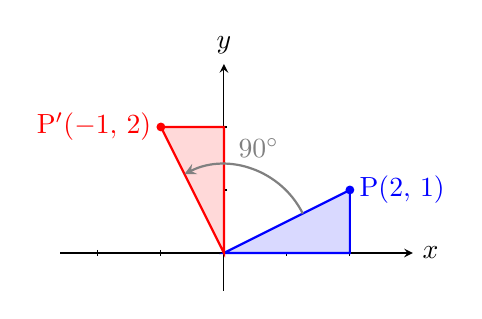
\begin{tikzpicture}[scale=0.8,>=stealth]
  \draw[->] (-2.6,0) -- (3,0) node[right] {$x$};
  \draw[->] (0,-0.6) -- (0,3) node[above] {$y$};
  \foreach \x in {-2,-1,1,2} \draw (\x,0.05) -- (\x,-0.05);
  \foreach \y in {1,2} \draw (0.05,\y) -- (-0.05,\y);
  % 元の三角形 O(0,0), P(2,1), Q(2,0)
  \filldraw[fill=blue!15,draw=blue,thick] (0,0) -- (2,1) -- (2,0) -- cycle;
  % 回転後 O, P'(-1,2), Q'(0,2)
  \filldraw[fill=red!15,draw=red,thick] (0,0) -- (-1,2) -- (0,2) -- cycle;
  \fill[blue] (2,1) circle (2pt) node[right] {P$(2,\,1)$};
  \fill[red] (-1,2) circle (2pt) node[left] {P$'(-1,\,2)$};
  % 原点を中心に、OP の向き（約26.6°）から OP' の向き（約116.6°）まで 90° の弧
  \draw[->,gray,thick] (26.57:1.4) arc (26.57:116.57:1.4);
  \node[gray] at (71.57:1.75) {$90^\circ$};
\end{tikzpicture}
